% четвертая часть

\section{Разработка программного обеспечения системы учета ресурсов}
\subsection{Назначение}
Основная задача разрабатываемой программы упростить учет и администрирование контроллеров и приборов учета, а также своевременный анализ данных, для выявления неисправных оборудований. Составления отчетов для ЖКХ.

Полный функционал программного обеспечения:
\begin{itemize}
	\item Добавление, редактирование и просмотр оборудований СКАУТ;
	\item Просмотр замененных КПУ и ПУ;
	\item Добавление, редактирование, замена и просмотр контроллеров приборов учета; 
	\item Просмотр истории редактирования КПУ; 
	\item Добавление, редактирование, замена и просмотр приборов учета; 
	\item Добавление стартовых значений; 
	\item Просмотр часовых показаний за выбранный период; 
	\item Просмотр истории редактирования ПУ;
	\item Просмотр приборов учета имеющих короткое замыкание или обрыв линии;
	\item Автоматический анализ данных на выявление проблемных счетчиков;
\end{itemize}

Программа включает 6 основных разделов.
\begin{enumerate}
	\item Раздел - Главное меню
	\item Раздел - СКАУТ
	\item Раздел - Контроллеры Приборов Учета
	\item Раздел - Приборы Учета
	\item Раздел - Контроль линии
	\item Раздел - Проблемные счетчики
\end{enumerate}

\subsection{Описание разделов программы}
\subsubsection{Главное меню}
Раздел «Главное меню» открывается при запуске программы. Отображаются две таблицы со списком замененных КПУ и ПУ. Из вкладки «Оборудование» можно перейти в разделы «СКАУТ», «КПУ», «ПУ». Из вкладки «Анализ данных» можно перейти в раздел «Контроль линии» и «Проблемные счетчики».

\subsubsection{СКАУТ}
Раздел «СКАУТ» открывается из главного меню, вкладки «Оборудование». Отображается список подъездов, где установлен СКАУТ. 
\begin{enumerate}
	\item Кнопка «Обновить» применяет выбранные фильтры к таблице;
	\item Кнопка «Добавить» открывает форму для заполнения данных для нового СКАУТА;
	\item Двойное нажатие на строчку из таблицы. Открывается полная информация по выбранному СКАУТу. При нажатии кнопки «КПУ» откроется список КПУ подключенных к данному СКАУТу;
\end{enumerate}

\subsubsection{КПУ или Контроллеры Приборов Учета}
Раздел «КПУ» открывается из главного меню, вкладки «Оборудование» и через нажатие на кнопку «КПУ» в форме «Информация о СКАУТ». Отображается список установленных КПУ.
\begin{enumerate}
	\item Кнопка «Обновить» применяет выбранные фильтры к таблице;
	\item Кнопка «Добавить» открывает форму для заполнения данных для нового КПУ;
	\item Двойное нажатие на строчку из таблицы. Открывается информация по выбранному КПУ. Можно переключиться на вкладку «История редактирования», где отображается таблица с информацией о редактировании данных выбранного КПУ. При нажатии кнопки «ПУ» откроется список ПУ подключенных к данному КПУ;
	\item Кнопка «Заменить». Используется, когда заменили установленный КПУ на другой. Если при замене на новом КПУ указали такие же импульсы, какие были на старом, и не требуется менять показания на всех ПУ подключенных к данному КПУ, тогда убираем галочку «с заменой стартовых значений». Если указали нулевые импульсы на все клеммы, то требуется заменить стартовые значения. Выбираем время и нажимаем обновить. Отобразятся показания, номера квартир и тип ПУ на выбранную дату для старого КПУ. Если на указанное время КПУ был неисправен и показания в БД не записывались, тогда отобразятся последние сохранившиеся данные;
\end{enumerate}	

\subsubsection{ПУ или Приборы Учета}
Раздел «ПУ» открывается из главного меню, вкладки «Оборудование» и через нажатие на кнопку «ПУ» в форме «Информация о КПУ». Отображается список установленных ПУ. 
\begin{enumerate}
	\item Кнопка «Обновить» применяет выбранные фильтры к таблице;
	\item Кнопка «Добавить» открывает форму для заполнения данных для нового ПУ. Если квартиры еще нету в БД, то откроется форма для добавления новой квартиры;
	\item Двойное нажатие на строчку из таблицы. Открывается информация по выбранному ПУ. Если нужно добавить дату установки и демонтажа, то нажать на кнопку «Дата установки отсутствует» и «Дата демонтажа отсутствует»;
	\item Вкладка «Информация». При нажатии кнопки «ПУ» откроется список ПУ подключенных к данному КПУ;
	\item Кнопка «Заменить». Используется, когда заменили установленный ПУ на другой. Выбираем время, когда сняли показания с нового ПУ и нажимаем «Установить импульсы на выбранную дату», чтобы автоматически заполнились имеющиеся импульсы на подключенной клемме. Если серийный номер нового ПУ уже имеется в БД, то покажется предупреждение об этом. Если ПУ нигде не установлен, то предложит продолжить замену;
	\item Вкладка «Стартовые значения». Отображается таблица с информацией о добавленных стартовых значения для выбранного ПУ. Можно добавить новое стартовое значение;
	\item Вкладка «Показания». Отображается таблица с часовыми показаниями выбранного ПУ. По умолчанию за последние сутки. Можно изменить временной промежуток и нажать кнопку «Показать»;
	\item Вкладка «История редактирования». Отображается таблица с информацией о редактировании данных выбранного ПУ;
\end{enumerate}
	
\subsubsection{Контроль линии}
Раздел «Контроль линии» открывается из главного меню, вкладки «Анализ данных». Отображается список проблемных ПУ за последние сутки. Если столбец line\_state = 1, тогда произошел обрыв линии или короткое замыкание на линии от ПУ до КПУ. Столбец empty = 1 означает что данные не обновились. 
\subsubsection{Проблемные счетчики}
Раздел «Проблемные счетчики» открывается из главного меню, вкладки «Анализ данных». Отображается список проблемных ПУ за последние трое суток. Пользователь может выбрать свой промежуток времени. При двойном нажатие на строчку из списка откроется информационное окно с удобными, для анализа показаний, графиками потребления всех видов ресурсов выбранной квартиры. 
\subsection{Разработка программы}
\subsubsection{PyQT5}
PyQt5 --- это набор Python-связей для фреймворка Qt5 от Digia. Набор PyQt5 доступен для Python 2.x и 3.x. В моей программе используется Python 3. Библиотека Qt – это одна из самых мощных GUI-библиотек. PyQt5 разработан компанией Riberbank Computing.\cite{Python}

PyQt5 реализован как комплект Python-модулей. Он включает в себя около 620 классов и 6000 функций и методов, включая:
\begin{enumerate}
	\item Существующий набор виджетов графического интерфейса;
	\item Стили виджетов;
	\item Доступ к базам данных с помощью SQL (ODBC, MySQL, PostgreSQL, Oracle);
	\item QScintilla, основанный на Scintilla виджет текстового редактора;
	\item Поддержку интернационализации (i18n);
	\item Парсер XML;
	\item Поддержку SVG;
	\item Интеграцию с WebKit, движком рендеринга HTML;
	\item Поддержку воспроизведения видео и аудио;
\end{enumerate}
Это мульти-платформенный инструментарий, который запускается на большинстве операционных систем, среди которых Unix, Windows и MacOS. PyQt5 реализован под двумя лицензиями. Разработчики могут выбрать между GPL и коммерческой лицензией.

PyQt также включает в себя Qt Designer (Qt Creator) — дизайнер графического интерфейса пользователя. Программа pyuic генерирует Python код из файлов, созданных в Qt Designer. Это делает PyQt очень полезным инструментом для быстрого прототипирования. Кроме того, можно добавлять новые графические элементы управления, написанные на Python, в Qt Designer.\cite{PyQt5}
\subsubsection{fdb}
FDB - это пакет библиотеки Python, реализующий поддержку Python Database API 2.0 для реляционной базы данных с открытым исходным кодом Firebird. В дополнение к минимальному набору функций стандартного API Python DB, FDB также предоставляет полный нативный (в старом стиле) клиентский API ядра базы данных и ряд дополнительных расширений и улучшений для удобного использования Firebird.\cite{fdb}

FDB разрабатывается в рамках с проектом Firebird, и используется внутренне как ключевой компонент для Firebird QA.\cite{firebird}

Доступ к базе данных осуществляется через объекты подключения. FDB предоставляет два конструктора для них:
\begin{enumerate}
	\item create\_database () --- создание базы данных данных;
	\item connect () --- создание подключения к базе данных;
\end{enumerate}
Для дальнейшего общение с базой нужно получить курсор. Пример добавления нового элемента в таблицу
\begin{MyCode}
import psycopg2
conn = psycopg2.connect(dbname='database', user='user', 
password='mypassword', host='localhost')
cur = conn.cursor()
cur.execute("insert into KPU (SER\_NUM, ADRESS) values (?,?)",
		(1784, 1))
conn.commit()
cur.close()
conn.close()
\end{MyCode}
\subsubsection{psycopg2}
PostgreSQL, пожалуй, это самая продвинутая реляционная база данных в мире Open Source Software. По своим функциональным возможностям она не уступает коммерческой БД Oracle и на голову выше собрата MySQL.\cite{psycopg}

В Python самой популярной библиотекой для работы с PostgreSQL является psycopg2. Эта библиотека написана на Си на основе libpq, соответствует стандарту DB-API 2.0. Основные методы DB-API, позволяющие полноценно работать с базой данных представлены на рис.~\ref{fig:pythondb-api}

\begin{figure}[H]
	\centering
	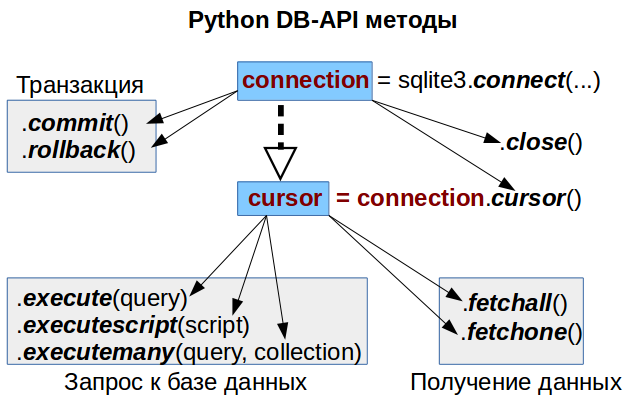
\includegraphics[width=0.7\linewidth]{pics/pythonDB-API}
	\caption{Python DB-API Методы}
	\label{fig:pythondb-api}
\end{figure}
 

